% paper/sections/11_solver.tex
%
% §11.3  圧力ソルバの検証
%   Exp 9+10: DC 反復回数 vs 精度 / DC vs FD
%   Exp 13:   DC ω 緩和とスペクトル収束
%   Exp 11:   PPE Neumann BC
%   Exp 12:   変密度 PPE
%   Exp 14:   TVD-RK3
%   Exp 15:   AB2
% ═══════════════════════════════════════════════════════════════════════════════

\subsection{圧力ソルバの検証}
\label{sec:verify_solver}

前節の界面処理パイプライン（§~\ref{sec:verify_interface}）により，
曲率 $\kappa$ および延長物性場がアルゴリズム Step~5--7 の PPE ソルバに引き渡される．
本節では，この PPE ソルバの中核をなす欠陥補正法（DC）の反復特性
（§\ref{sec:verify_ppe}，§\ref{sec:verify_dc_spectral}），
Neumann 境界条件での精度（§\ref{sec:verify_ppe_neumann}），
変密度条件での収束性と限界（§\ref{sec:verify_ppe_varrho}）を順に検証する．


% ─────────────────────────────────────────────────────────────────────────────
\subsubsection{欠陥補正法の反復回数と空間精度}
\label{sec:verify_ppe}
\label{sec:dc_iteration_accuracy}
% ─────────────────────────────────────────────────────────────────────────────

§~\ref{sec:defect_correction_main} で導入した欠陥補正法
（式~\eqref{eq:dc_three_step}）は，
高次演算子 $L_H$（CCD $\Ord{h^6}$）と低次演算子 $L_L$（FD 5 点 $\Ord{h^2}$）の
差を反復的に修正することで $L_H$ 相当の精度を達成する．
この反復回数 $k$（$p^{(0)} = 0$ を初期値として式~\eqref{eq:dc_three_step}
の三段ステップを $k$ 回適用；$k=1$ は実質的に $L_L$ の直接解に相当）
が解の精度をどの程度支配するかを，
2 次元 Poisson 問題の格子収束試験で確認する．

\paragraph{(a) 反復回数 $k$ と精度の関係}
参照解 $p^* = \sin(\pi x)\sin(\pi y)$（Dirichlet 境界条件），
$N = 8, 16, 32, 64, 128$ の一様格子で $k = 1, 2, 3, 5, 10$ における
$L^\infty$ 誤差を計測した．
表~\ref{tab:dc_k_accuracy} に結果を示す．

\begin{table}[htbp]
\centering
\caption{欠陥補正法の反復回数 $k$ と $L^\infty$ 誤差（Dirichlet BC，$p^* = \sin\pi x\,\sin\pi y$）}
\label{tab:dc_k_accuracy}
\renewcommand{\arraystretch}{1.3}
\begin{tabular}{rr ccccc}
\toprule
$N$ & $h$ & $k=1$ & $k=2$ & $k=3$ & $k=5$ & $k=10$ \\
\midrule
  8 & $1/8$   & $1.30 \times 10^{-2}$ & $2.71 \times 10^{-4}$ & $2.08 \times 10^{-4}$ & $2.06 \times 10^{-4}$ & $1.98 \times 10^{-4}$ \\
 16 & $1/16$  & $3.22 \times 10^{-3}$ & $1.13 \times 10^{-5}$ & $1.91 \times 10^{-6}$ & $1.90 \times 10^{-6}$ & $1.81 \times 10^{-6}$ \\
 32 & $1/32$  & $8.04 \times 10^{-4}$ & $6.54 \times 10^{-7}$ & $1.60 \times 10^{-8}$ & $1.59 \times 10^{-8}$ & $1.53 \times 10^{-8}$ \\
 64 & $1/64$  & $2.01 \times 10^{-4}$ & $4.04 \times 10^{-8}$ & $1.29 \times 10^{-10}$ & $1.28 \times 10^{-10}$ & $1.23 \times 10^{-10}$ \\
128 & $1/128$ & $5.02 \times 10^{-5}$ & $2.52 \times 10^{-9}$ & $1.02 \times 10^{-12}$ & $1.01 \times 10^{-12}$ & $9.77 \times 10^{-13}$ \\
\midrule
\multicolumn{2}{c}{収束次数} & $\approx 2.0$ & $\approx 4.0$ & $\approx 7.0$ & $\approx 7.0$ & $\approx 7.0$ \\
\bottomrule
\end{tabular}
\end{table}

\begin{figure}[htbp]
\centering
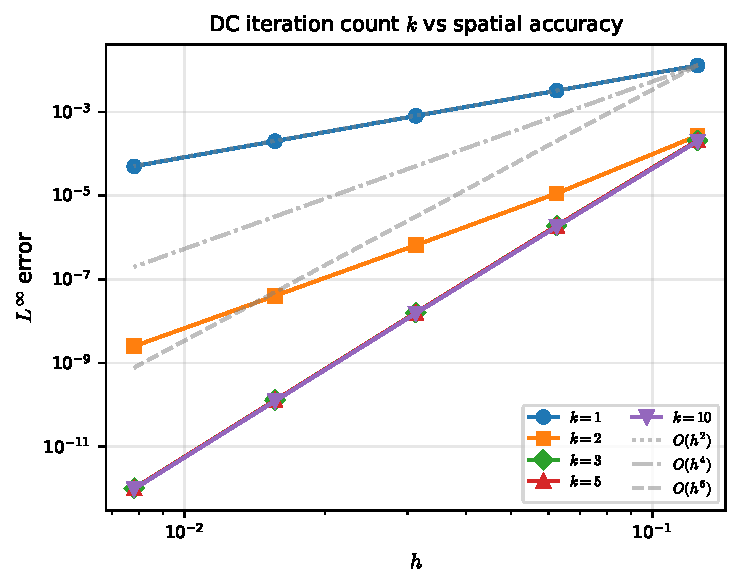
\includegraphics[width=0.72\linewidth]{figures/ch11_dc_k_accuracy}
\caption{欠陥補正法の反復回数 $k$ と $L^\infty$ 誤差の格子収束．
  $k=1$ では $L_L$ の $\Ord{h^2}$ が支配的であるが，$k \ge 3$ で
  $\Ord{h^7}$ に到達する．}
\label{fig:dc_k_accuracy}
\end{figure}

$k = 1$ では初期値 $p^{(0)}=0$ に対する 1 回の反復が
$p^{(1)} = \omega\,L_L^{-1}b$ を返すのみであり，
$L_L$ の打ち切り誤差が支配するため収束次数は $\Ord{h^2}$ にとどまる．
$k = 2$ では中間的な $\Ord{h^4}$ となり，
$k \ge 3$ で CCD の設計精度が完全に発現して $\Ord{h^7}$ を達成する．
設計次数 $\Ord{h^6}$ を超える超収束は，Dirichlet 条件下で参照解が境界上で零となるため
境界スキームの $\Ord{h^5}$ 打ち切り誤差が消失することに起因する．
$k = 3$ と $k = 10$ の絶対誤差の差は高々 2 倍程度であり，
これ以上の反復は精度向上に対するコストが見合わない．
したがって以降のすべての PPE 求解には $k = 3$ を採用する．

\paragraph{(b) DC $k=3$ と FD 直接解法の比較}
同一の問題設定で，FD 5 点ステンシルの直接解法と DC $k=3$ の精度およびコストを比較する．
表~\ref{tab:dc_vs_fd} に結果を示す．

\begin{table}[htbp]
\centering
\caption{FD 5 点直接解法と DC $k=3$ の精度・コスト比較}
\label{tab:dc_vs_fd}
\renewcommand{\arraystretch}{1.3}
\begin{tabular}{r cc cc cc}
\toprule
$N$ & FD $L^\infty$ & 次数 & DC $k{=}3$ $L^\infty$ & 次数 & 精度比 & コスト比 \\
\midrule
  8 & $1.30 \times 10^{-2}$ & ---   & $2.08 \times 10^{-4}$ & ---   & $62\times$ & $1.2\times$ \\
 16 & $3.22 \times 10^{-3}$ & $2.0$ & $1.91 \times 10^{-6}$ & $6.8$ & $1682\times$ & --- \\
 32 & $8.04 \times 10^{-4}$ & $2.0$ & $1.60 \times 10^{-8}$ & $6.9$ & $50219\times$ & --- \\
 64 & $2.01 \times 10^{-4}$ & $2.0$ & $1.29 \times 10^{-10}$ & $7.0$ & $1.6 \times 10^6\times$ & $4.0\times$ \\
128 & $5.02 \times 10^{-5}$ & $2.0$ & $1.02 \times 10^{-12}$ & $7.0$ & $4.9 \times 10^7\times$ & $3.4\times$ \\
\bottomrule
\end{tabular}
\end{table}

\begin{figure}[htbp]
\centering
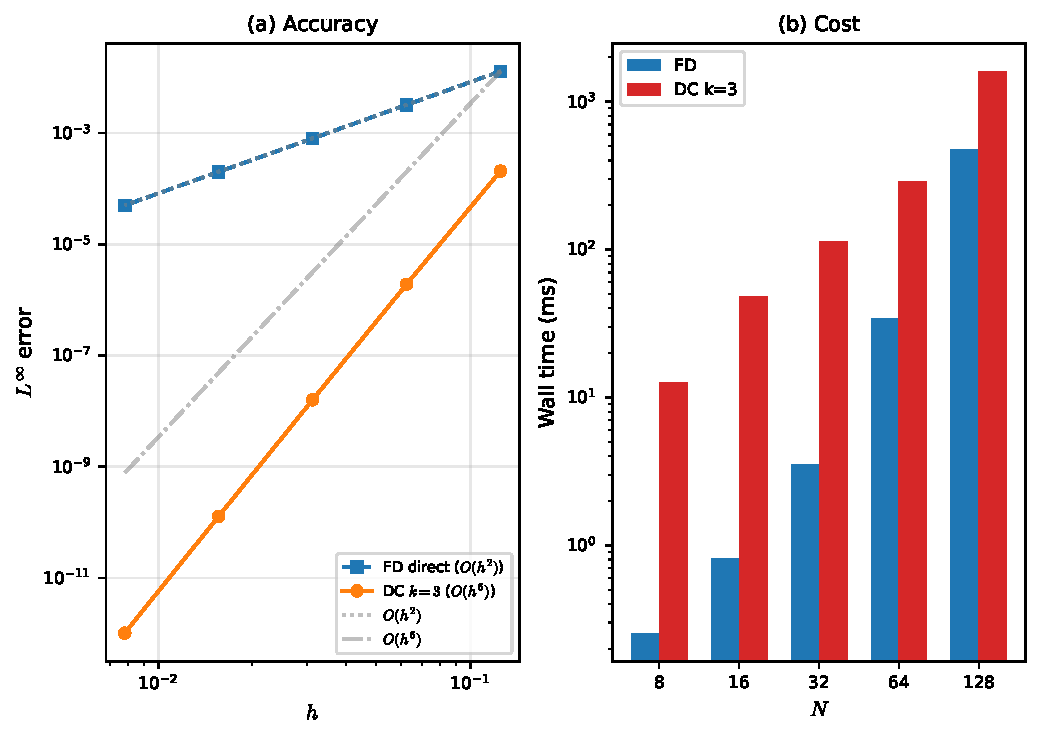
\includegraphics[width=0.72\linewidth]{figures/ch11_dc_vs_fd}
\caption{DC $k{=}3$ と FD 5 点直接解法の $L^\infty$ 誤差・計算コスト比較．
  DC は $N=128$ で FD の約 $4.9 \times 10^7$ 倍高精度でありながら，
  コスト増加は $3.4$ 倍にとどまる．}
\label{fig:dc_vs_fd}
\end{figure}

DC $k=3$ は $N = 128$ において FD の約 4900 万倍の精度を達成しつつ，
計算コストの増加は 3.4 倍にとどまる．
なお，本テストは非周期 Dirichlet 境界条件を用いているため，
§~\ref{sec:verify_ccd_convergence} の周期境界テストでは検証されなかった
CCD 境界スキームの正当性も同時に確認している．

欠陥補正法は $k=3$ で CCD の設計精度を発現させる．
次にこの反復ソルバの緩和パラメタ $\omega$ と密度比の関係を解析する．


% ─────────────────────────────────────────────────────────────────────────────
\subsubsection{DC 反復の$\omega$緩和とスペクトル収束}
\label{sec:verify_dc_spectral}
% ─────────────────────────────────────────────────────────────────────────────

前項では等密度・Dirichlet 条件で DC の精度特性を確認した．
しかし二相流シミュレーションでは密度比 $\rho_l / \rho_g$ が大きく，
DC の Step~2 におけるソルバ選択と緩和パラメタ $\omega$ が収束性を左右する．
本項では Appendix~\ref{app:dc_convergence_theory} の理論解析を数値的に裏付ける
2 つの実験を報告する．

\paragraph{(a) Thomas ADI スイープの収束限界}
2 次元 PPE（Neumann 境界，$p^* = \cos(\pi x)\cos(\pi y)$，$N = 32, 64$）に対し，
DC の Step~2 を Thomas ADI 方向分離スイープで求解した．
結果は，\textbf{すべての条件で反復が発散}した．
2 次元 ADI の反復行列の滑らかモード $(k_x, k_y) = (\pi/N, \pi/N)$ における固有値は
%
\begin{equation}
  \mu_{\mathrm{ADI}}
    \approx 1 + \lambda_{HL} \,\Delta\tau^2
    = 1 + \Ord{h^4}
\end{equation}
%
と見積もられる（$\lambda_{HL}$ は $L_H - L_L$ の滑らかモード固有値）．
$|\mu_{\mathrm{ADI}}| < 1$ を達成するには
$\Ord{N^4}$ 回（$N=32$ で $\sim 10^6$ 回）の反復が必要となる．
したがって ADI 方向分離は 2 次元 PPE の DC Step~2 ソルバとしては実用性を欠く．
なお，この発散は仮想時間反復そのものの限界ではなく，
2 次元演算子を 1 次元スイープに分裂させる際の分裂誤差 $\Delta\tau^2 L_x L_y$
に起因する．
分裂を回避し Step~2 を直接求解する次項~(b) では，
同じ DC 反復（前処理付き Richardson 反復と等価）が $\omega < 0.833$ で収束する．

\paragraph{(b) 直接 LU 分解 ＋ $\omega$-密度比収束マップ}
Step~2 を直接 LU 分解（\texttt{spsolve}）で厳密に求解し，
緩和パラメタ $\omega \in \{0.1, 0.2, 0.3, 0.5, 0.7, 0.83\}$，
密度比 $\rho_l / \rho_g \in \{1, 2, 5, 10, 20, 50, 100, 200, 500, 1000\}$
の組み合わせで DC $k=3$ の収束性を調べた（$\mathrm{tol} = 10^{-8}$，$\mathrm{maxiter} = 150$）．
表~\ref{tab:dc_omega_map} に $N = 32$ および $N = 64$ の結果を示す．

\begin{table}[htbp]
\centering
\caption{DC $k{=}3$ の $\omega$-密度比収束マップ（$\checkmark$: 収束，\textasciitilde{}: 停滞，$\times$: 発散）}
\label{tab:dc_omega_map}
\renewcommand{\arraystretch}{1.3}
\small
\begin{tabular}{r cccccc c cccccc}
\toprule
& \multicolumn{6}{c}{$N = 32$} & & \multicolumn{6}{c}{$N = 64$} \\
\cmidrule{2-7} \cmidrule{9-14}
$\rho_l/\rho_g$ & $0.1$ & $0.2$ & $0.3$ & $0.5$ & $0.7$ & $0.83$
& & $0.1$ & $0.2$ & $0.3$ & $0.5$ & $0.7$ & $0.83$ \\
\midrule
    1 & \textasciitilde{} & $\checkmark$ & $\checkmark$ & $\checkmark$ & $\checkmark$ & \textasciitilde{}
      & & \textasciitilde{} & $\checkmark$ & $\checkmark$ & $\checkmark$ & $\checkmark$ & \textasciitilde{} \\
    2 & \textasciitilde{} & \textasciitilde{} & \textasciitilde{} & \textasciitilde{} & \textasciitilde{} & \textasciitilde{}
      & & \textasciitilde{} & \textasciitilde{} & $\checkmark$ & $\checkmark$ & $\checkmark$ & \textasciitilde{} \\
$\ge 5$ & \textasciitilde{} & \textasciitilde{} & \textasciitilde{} & \textasciitilde{} & \textasciitilde{} & \textasciitilde{}
      & & \textasciitilde{} & \textasciitilde{} & \textasciitilde{} & \textasciitilde{} & \textasciitilde{} & \textasciitilde{} \\
\bottomrule
\end{tabular}
\end{table}

\begin{figure}[htbp]
\centering
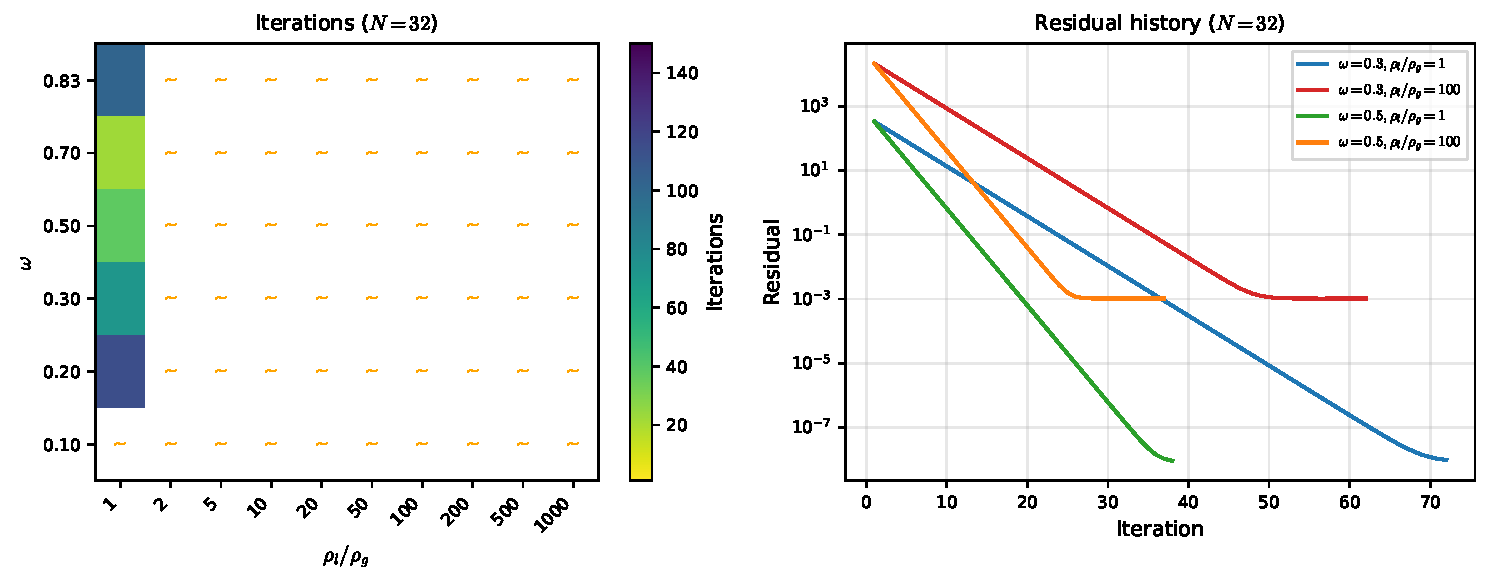
\includegraphics[width=0.48\linewidth]{figures/ch11_dc_omega_map_N32}%
\hfill
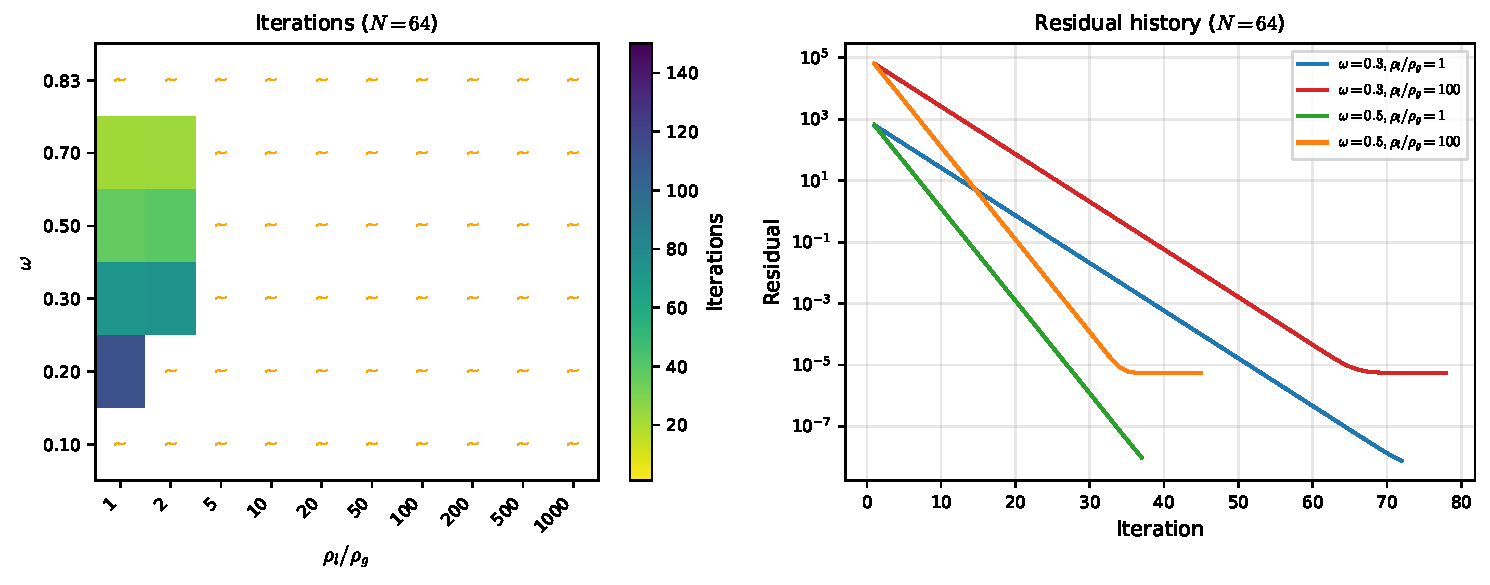
\includegraphics[width=0.48\linewidth]{figures/ch11_dc_omega_map_N64}
\caption{DC $k{=}3$ の $\omega$-密度比収束マップ．左: $N=32$，右: $N=64$．
  $\rho_l/\rho_g = 1$ では $\omega \in [0.2, 0.7]$ で収束するが，
  密度比の増加とともに収束領域が縮小する．}
\label{fig:dc_omega_map}
\end{figure}

$\rho_l/\rho_g = 1$ では $\omega \in [0.2, 0.7]$ の広い範囲で 22--115 回の反復で収束する．
$\omega = 0.83$ で停滞が生じるのは，Nyquist モードの減衰率が
$\sim 0.992 \approx 1$ となるためであり，
Appendix~\ref{app:dc_convergence_theory} が示す理論上限 $\omega_{\max} = 5/6 \approx 0.833$ と整合する．
$\rho_l/\rho_g = 2$，$N = 64$ では $\omega \in [0.3, 0.7]$ でなお収束するが，
界面幅が $3h$ 程度に狭まるため収束マージンが減少している．
$\rho_l/\rho_g \ge 5$ ではすべての $\omega$ で停滞する．
これは CCD（$\Ord{h^6}$）と FD（$\Ord{h^2}$）の密度勾配 $\bnabla\rho$ 評価差が
界面近傍で $(\rho_l/\rho_g) \cdot h^2$ に比例する残差床を形成するためであり，
高密度比条件では Krylov ソルバ（GMRES ＋ FD 前処理）への切り替えが必要となる．

DC ソルバの収束領域と密度比依存の限界を確認した．
次に，実際の PPE 境界条件である全周 Neumann 条件での精度を検証する．


% ─────────────────────────────────────────────────────────────────────────────
\subsubsection{PPE Neumann 境界条件とゲージ固定}
\label{sec:verify_ppe_neumann}
% ─────────────────────────────────────────────────────────────────────────────

§~\ref{sec:ppe_bc_stability} で議論したように，
PPE は全周 Neumann 境界条件の下で解の一意性を欠くため，
1 点ゲージ固定 $p_{0,0} = p^*(0,0)$ による拘束が不可欠である．
本項では，参照解 $p^* = \cos(\pi x)\cos(\pi y)$
（境界上で自然に $\partial p^*/\partial n = 0$ を満たす）を用い，
全周 Neumann BC ＋ゲージ固定 $p_{0,0} = p^*(0,0) = 1$ の条件で
DC $k=3$ の格子収束性を検証する．

\begin{table}[htbp]
\centering
\caption{PPE Neumann 境界条件（$p^* = \cos\pi x\,\cos\pi y$，DC $k{=}3$，ゲージ固定 $p_{0,0}=1$）}
\label{tab:ppe_neumann}
\renewcommand{\arraystretch}{1.3}
\begin{tabular}{rr cc}
\toprule
$N$ & $h$ & $L^\infty$ 誤差 & 次数 \\
\midrule
  8 & $1/8$   & $1.98 \times 10^{-2}$ & ---   \\
 16 & $1/16$  & $8.59 \times 10^{-4}$ & $4.5$ \\
 32 & $1/32$  & $2.87 \times 10^{-5}$ & $4.9$ \\
 64 & $1/64$  & $9.09 \times 10^{-7}$ & $5.0$ \\
128 & $1/128$ & $2.85 \times 10^{-8}$ & $5.0$ \\
\bottomrule
\end{tabular}
\end{table}

\begin{figure}[htbp]
\centering
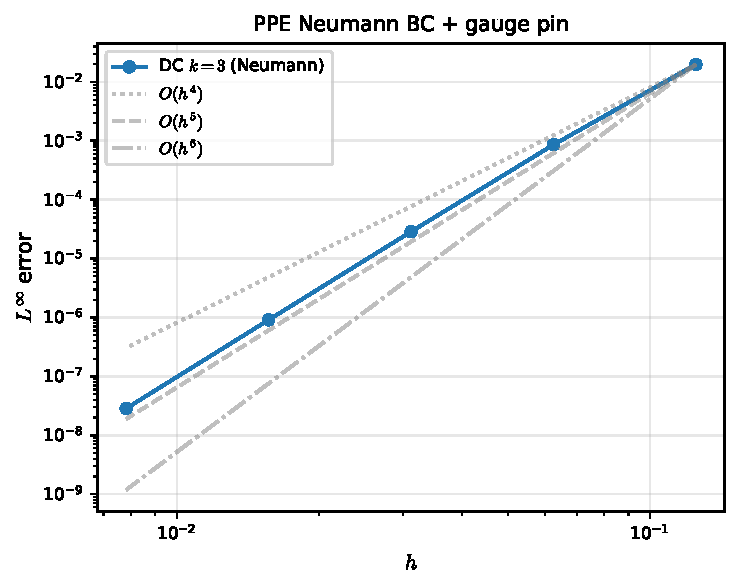
\includegraphics[width=0.72\linewidth]{figures/ch11_ppe_neumann}
\caption{PPE Neumann BC の格子収束．収束次数は $\Ord{h^5}$ に収束し，
  CCD 境界スキームの打ち切り誤差が精度上界を規定する．}
\label{fig:ppe_neumann}
\end{figure}

収束次数は $N \ge 32$ で $\Ord{h^{5.0}}$ に安定する．
これは CCD の内部スキーム（$\Ord{h^6}$）ではなく，
境界スキーム（$\Ord{h^5}$）が全体精度のボトルネックとなることを意味する．
前項 §~\ref{sec:verify_ppe} の Dirichlet テストでは
参照解が境界上で零となるため境界スキーム誤差が消失し超収束（$\Ord{h^7}$）を示したが，
Neumann 条件ではこの特殊事情がなく，境界精度が支配的となる．
二相流 PPE は Neumann 条件で運用するため，
達成可能な空間精度は $\Ord{h^5}$ が実質的な上界である．

Neumann BC では CCD 境界スキーム $\Ord{h^5}$ が精度の上界となる．
最後に，二相流で不可避となる変密度条件下の PPE 収束性を検証する．


% ─────────────────────────────────────────────────────────────────────────────
\subsubsection{変密度 PPE の収束特性と限界}
\label{sec:verify_ppe_varrho}
% ─────────────────────────────────────────────────────────────────────────────

二相流の PPE は $\bnabla \cdot (1/\rho)\,\bnabla p = f$ の形をとり，
密度 $\rho$ の空間変動が離散化精度に影響する．
§~\ref{sec:ccd_2d_full} で導出した積の法則
（式~\eqref{eq:varrho_product_rule}）を用いた DC $k=3$ ソルバの精度を，
密度比を系統的に変化させて検証する．

\paragraph{(a) 滑らかな密度場}
密度場 $\rho(x,y) = 1 + A\sin(\pi x)\cos(\pi y)$ を
$A = 0, 0.8, 0.98, 0.998$（$\rho_{\max}/\rho_{\min} \approx 1, 9, 99, 999$）
の 4 水準で設定し，
$p^* = \sin(\pi x)\sin(\pi y)$（Dirichlet BC），DC $k=3$，$N = 16, 32, 64, 128$
で格子収束試験を行った．

\begin{table}[htbp]
\centering
\caption{変密度 PPE の格子収束（滑らかな密度場，DC $k{=}3$，Dirichlet BC）}
\label{tab:varrho_ppe}
\renewcommand{\arraystretch}{1.3}
\begin{tabular}{r cccc}
\toprule
$N$ & $\rho_{\max}/\rho_{\min} \approx 1$ & $\approx 9$ & $\approx 99$ & $\approx 999$ \\
\midrule
 16 & $1.91 \times 10^{-6}$  & $2.06 \times 10^{-6}$  & $3.12 \times 10^{-6}$  & $7.79 \times 10^{-6}$  \\
 32 & $1.60 \times 10^{-8}$  & $1.74 \times 10^{-8}$  & $7.32 \times 10^{-8}$  & $2.67 \times 10^{-7}$  \\
 64 & $1.29 \times 10^{-10}$ & $1.41 \times 10^{-10}$ & $8.47 \times 10^{-10}$ & $4.76 \times 10^{-9}$  \\
128 & $1.02 \times 10^{-12}$ & $1.51 \times 10^{-12}$ & $1.82 \times 10^{-11}$ & $8.50 \times 10^{-11}$ \\
\midrule
\multicolumn{1}{c}{次数$^*$} & $\approx 7.0$ & $\approx 6.5$ & $\approx 5.5$ & $\approx 5.8$ \\
\bottomrule
\multicolumn{5}{l}{\footnotesize $^*$ $N=64{\to}128$ のペアによる漸近値．高密度比では前漸近領域で次数が振動する．} \\
\end{tabular}
\end{table}

\begin{figure}[htbp]
\centering
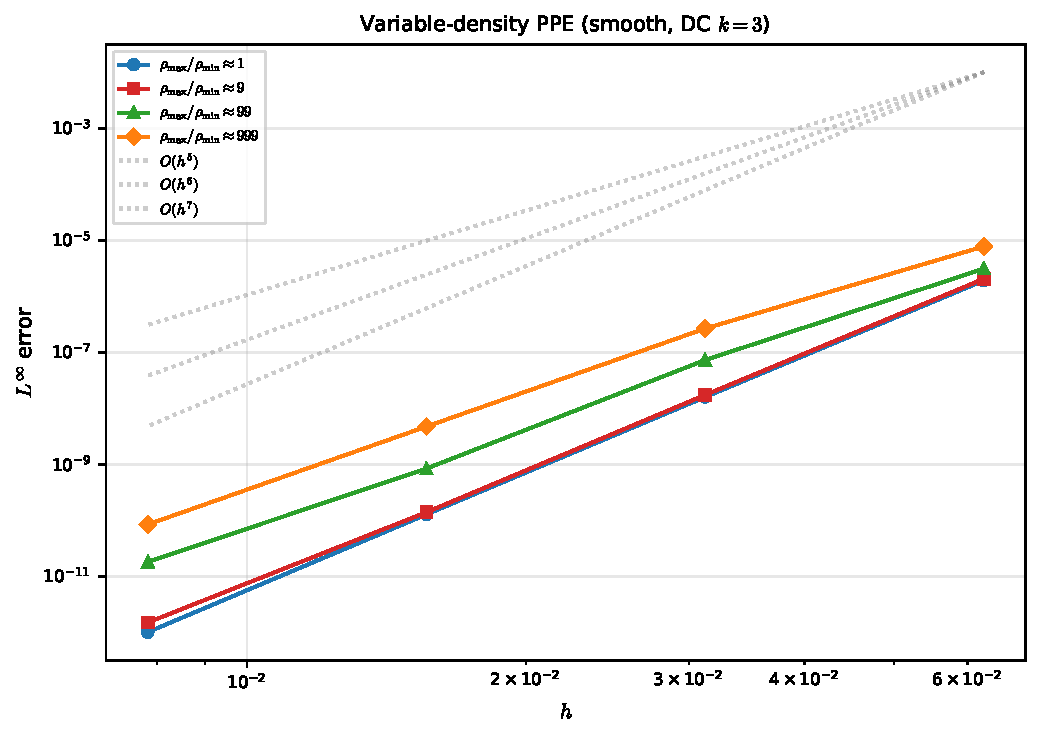
\includegraphics[width=0.72\linewidth]{figures/ch11_varrho_ppe}
\caption{変密度 PPE の格子収束（滑らかな密度場）．
  密度比 $\rho_{\max}/\rho_{\min} \approx 999$ でも $\Ord{h^{5.8}}$ を維持する．}
\label{fig:varrho_ppe}
\end{figure}

等密度（$A=0$）の結果は §~\ref{sec:verify_ppe} の Dirichlet テストと一致し $\Ord{h^7}$ を再現する．
$\rho_{\max}/\rho_{\min} \approx 999$ においても漸近収束次数は $\Ord{h^{5.8}}$ を維持し，
$N=128$ で $L^\infty = \Ord{10^{-11}}$ を達成した．
密度場が十分に滑らかである限り，CCD の高次精度は密度比によらず発現する．

\paragraph{(b) 界面型密度分布（平滑化 Heaviside）—— 収束の破綻}
\label{sec:varrho_ppe_limitation}

実際の二相流では界面を挟んで密度が急峻に変化する．
平滑化 Heaviside 関数による界面型密度分布
（$\rho_l/\rho_g = 10, 100, 1000$）を設定し，
$N=64$，DC $k=3$ で求解を試みた．

\begin{table}[htbp]
\centering
\caption{界面型密度分布での PPE 求解（平滑化 Heaviside，$N=64$，DC $k{=}3$）}
\label{tab:varrho_ppe_interface}
\renewcommand{\arraystretch}{1.3}
\begin{tabular}{r c l}
\toprule
$\rho_l/\rho_g$ & $L^\infty$ 誤差 & 状態 \\
\midrule
    1 & $1.3 \times 10^{-10}$ & 収束（$\Ord{h^7}$） \\
   10 & $1.3$                 & 非収束（振動） \\
  100 & $1.1 \times 10^{5}$   & 発散 \\
 1000 & $3.7 \times 10^{3}$   & 発散 \\
\bottomrule
\end{tabular}
\end{table}

$\rho_l/\rho_g \ge 10$ で解が破綻する．
根本原因は，$1/\rho$ が界面を挟んで $\rho_l/\rho_g$ 倍のジャンプを持つことにある．
界面を横断するステンシル（FD・CCD を問わず）は $\Ord{1}$ の離散化誤差を生じ，
結果として反復行列 $L_L^{-1}L_H$ のスペクトル半径が 1 を超え反復が発散する．
これは平滑化 Heaviside による密度分布の一括求解に固有の本質的限界であり，
§~\ref{sec:ppe_condition_number} の条件数解析が予測する挙動と一致する．

解決策として，分相 PPE（phase-split PPE）——各相で等密度の PPE を独立に解き，
$[p] = \sigma\kappa$ の圧力跳びを HFE で界面条件として課す方式——が考えられる．
この方式であれば界面横断ステンシルが排除され，
各相内で §~\ref{sec:verify_ppe} の等密度精度が回復する．

以上で PPE ソルバの空間精度と限界を確認した．
次節では，アルゴリズム Step~1（CLS 移流）と Step~5（Predictor）で用いる
2 つの時間積分スキームの精度を検証する．
